% !TEX root = ../main.tex
\begin{figure}[t]
\vspace{-0.2in}
\centering
\iflatexml
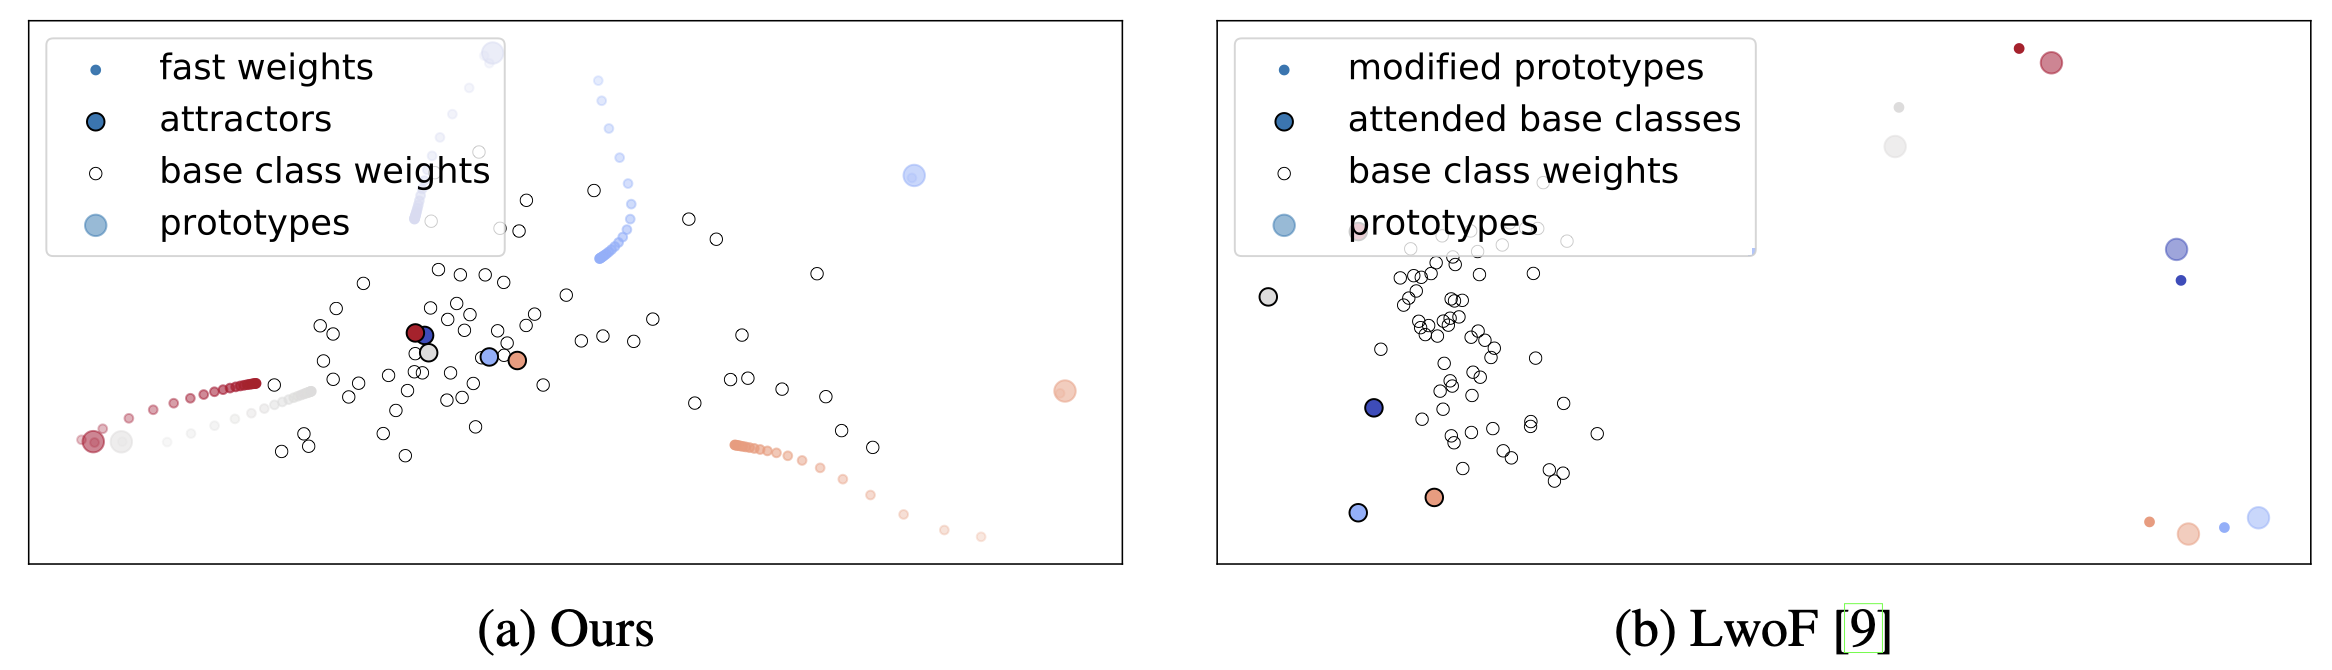
\includegraphics[width=6\textwidth]{figures/attractor_progress.png}
\else
\begin{minipage}[c]{\textwidth}
\centering
\begin{small}
\begin{tabular}{cc}
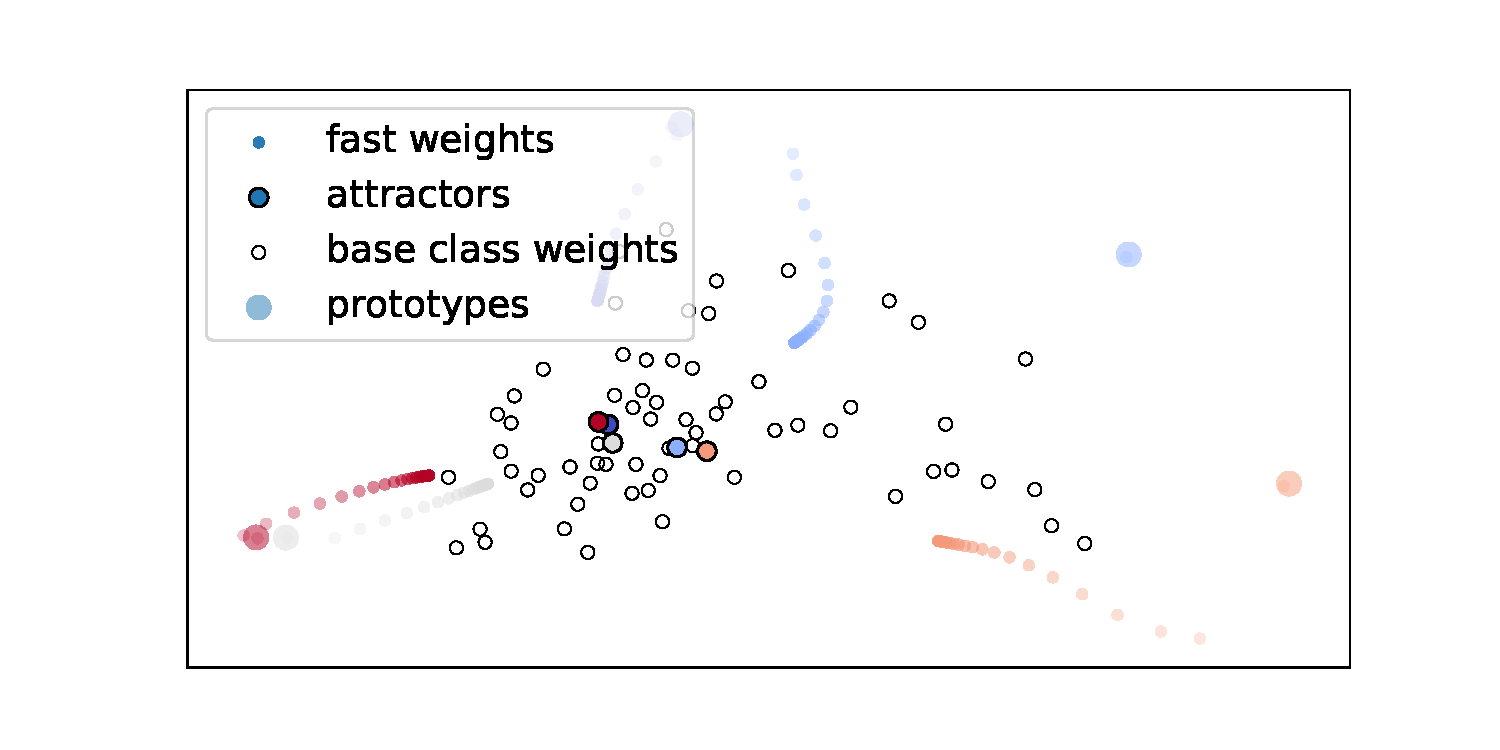
\includegraphics[width=0.47\textwidth,trim={2.8cm 1cm 2.5cm 1cm},clip]{figures/attractor_progress_9.pdf} & 
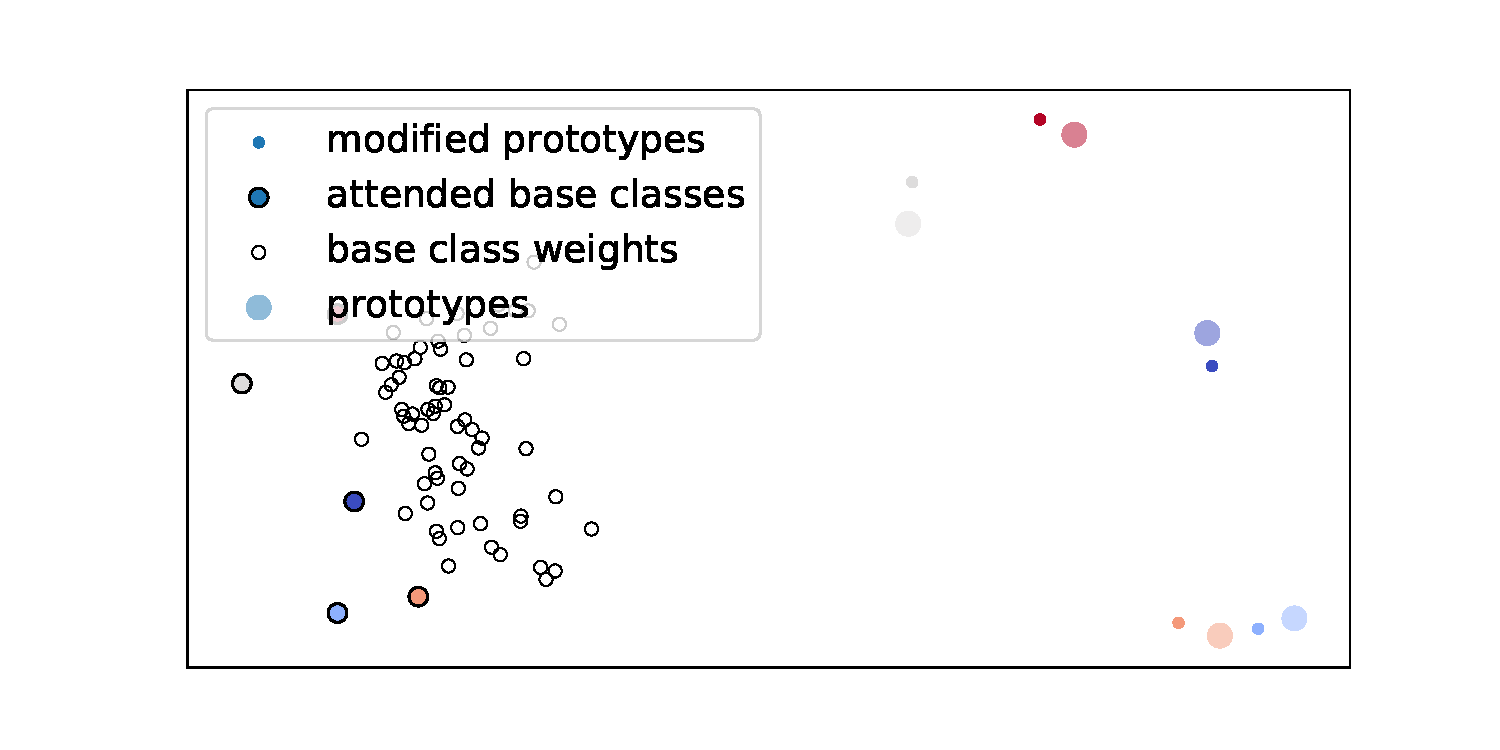
\includegraphics[width=0.47\textwidth,trim={2.8cm 1cm 2.5cm 1cm},clip]{figures/lwof_progress_9.pdf}\\
(a) Ours & (b) LwoF \cite{lwof}
\end{tabular}
\end{small}
\end{minipage}
\fi
\caption{Visualization of a 5-shot 64+5-way episode using PCA. 
\textbf{Left:} Our attractor model learns to
``pull'' prototypes (large colored circles) towards base class weights (white circles). We visualize the trajectories during episodic training; \textbf{Right:} Dynamic few-shot learning without
forgetting \cite{lwof}.}
\label{fig:vizproc}
\vspace{-0.1in}
\end{figure}